%форматирование размера документа
\documentclass[11pt, a4paper, twocolumn]{book}
\usepackage[left=38mm,right=30mm, top=3cm,bottom=5.4cm,bindingoffset=0cm]{geometry}
\columnsep 10mm
\usepackage{fancyhdr}
\pagestyle{fancy}
\usepackage{multicol}

%работа с колонтитулами
\renewcommand{\headrulewidth}{0 pt}
\cfoot{}
\footskip=5mm

%текст, шрифты
\usepackage[utf8]{inputenc}
\usepackage[russian]{babel}
\usepackage{setspace}
\setstretch{0,9}

%\raise 2mm\vbox{
%работа с картинками и таблицами
\usepackage{graphicx}
\graphicspath{{images/}}
\usepackage{wrapfig}
\usepackage{tabularx}

\begin{document}
	\thispagestyle{empty}

\onecolumn
\begin{center}
	\
\vspace{2 cm}

\huge Национальный исследовательский университет компьютерных технологий, механики и оптики
\vspace{0.5cm}

\Huge Факультет ПИиКТ


\vspace{3cm}
\huge Информатика. Лабораторная работа №7.
\vspace{0.2cm}

\LARGE Вариант №
\end{center}
\vspace{4 cm}

\begin{flushright}
\Large

	Работу выполнил: Кулаков Н.\,В.
	\smallskip
	
	Группа: P3130
	\smallskip
	
	Преподаватель: Калинин И.\,В.
	\smallskip
	
	Город: Санкт-Петербург
	\vspace{2cm}
	
\centering2020 год
\end{flushright}


	\newpage
	
	\setcounter{page}{16}
	\fancyfoot[LE]{\footnotesize\thepage}
\fancyfoot[LO]{\footnotesize 3~~\scriptsize Квант №3}
\fancyfoot[RO]{\footnotesize\thepage}
\twocolumn
\begin{footnotesize}
\noindent Рис.\,2. В $N$ имеется всего $2^4$ подмножеств:

\noindent$C^0_4 = 1$ 0-подмножество (пустое)
 
\vspace{4mm}
\noindent $C^1_4 = 4$ подмножества,

\vspace{10mm}
\noindent $C^2_4 = 6$  подмножеств,

\vspace{13mm}
\noindent $C^3_4 = 3$ подмножеств,

\vspace{10mm}
\noindent $C^4_4 = 1$ подмножество (все множество $N$).
\end{footnotesize}
\vspace{5mm}

Обозначим число $k$-подмножеств в множестве из $n$ элементов через $C^k_n$~*).

Числа $C^k_n$ (их называют биномиальными коэффициетами) обладают целым рядом любопытных свойств. О многие из них было рассказано в статье Д.\,Б.~Фукса и М.\,Б.~Фукса «Арифметика биномиальных коэффициентов»(«Квант», №6, 1970). В этой статье было доказано, что 
\begin{equation}
	C^k_n = C^{k-1}_{n-1} + C^k_{n-1},
\end{equation}

\noindent и с помощью метода математической индукции получена формула для $C^k_n$:

\begin{equation}
	C^k_n = \frac{n!}{k!(n - k)!}{\ast\ast}).
\end{equation}

Оба утверждения были выведены из равенства $ C^k_n = \sum^{n}_{i=0}C^i_nx^i $, но их можно доказать и комбинаторными рассуждениями.

Чтобы доказать, например, равенство $ (1) $, зафиксируем один элемент $a$ из $ N $ и разобьем все $ k $-подмножества в $ N $ на два класса: содержащие $a$

\noindent\rule{1.8cm}{1px}
\vspace{2mm}

\begin{footnotesize}
*)\,Это число называют числом сочетаний из $ n $ элементов по $ k $ ($ C $ - первая буква французского слова combinaison -- сочетание).

**)\,Через $n!$ обозначают произведение всех натуральных чисел от 1 до $ n $. Например: $ 6!= 1\cdot2\cdot3\cdot4\cdot5\cdot6=720. $
\end{footnotesize}

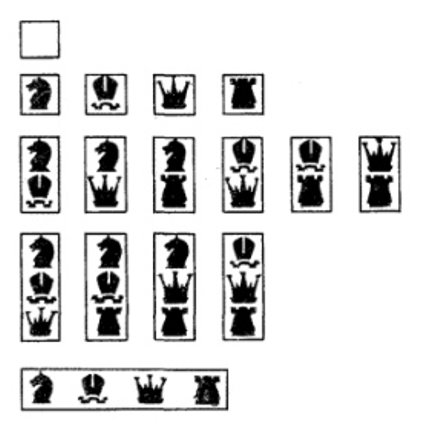
\includegraphics[width=\linewidth]{first.png}

 и не содержащие $a$. Проверьте что число подмножеств первого класса равно $C^{k-1}_{n-1}$, а число подмножеств второго класса равно $C^k_{n-1}$. Так как каждое $k$-подмножество принадлежит либо первому, либо второму классу, общее число всех $k$-подмножеств равно $C^k_n$, то равенство $ (1) $ доказано.

Чтобы вывести формулу $ (2) $, выясним сначал, как получаются $k$-подмножества из $(k-1)$-подмножеств. Ясно, что для этого надо к $(k-1)$-подмножествам присоединить не входящие в них элементы. Так как все множество $N$ содержит $n$ элементов, то в данное $(k-1)$-подмножество не входит $n-(k-1)$ элементов. Значит, из каждого $(k - 1)$-подмножества можно получить $n - k + 1$ различных $k$-подмножеств. Но одно и то же $k$-подмножество может быть получено из различных $(k - 1)$-подмножеств - мы не знаем, какой из $k$ элементов оказался присоединенным в последнюю очередь. Иными словами, любое $k$-подмножество может быть получено $k$ различными способами из $(k - 1)$-подмножеств. Поэтому общее число $k$-подмножеств в $k$ раз меньше, чем $(n - k +1)~ C^{k-1}_n$. Итак,
\[C^k_n = \frac{n-k+1}{k}C^{k-1}_{n}~.\]
Пользуясь этой формулой и методом


\begin{figure}[t]
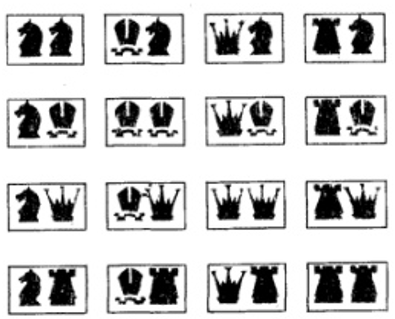
\includegraphics[width=\linewidth]{second.png}
\footnotesize
Рис.\,3. Существует $4^2 = 16$ 2-слов, составленных из элементов множества $N$.
\end{figure}

\noindent математической индукции, легко доказать и формулу $ (2) $.

\textbf{3. k-слова}. Снова возьмем в руки мешок с элементами множества $N$, но на этот раз будем вытаскивать элементы не сразу, а по очереди. Сначала вынем один элемент, обозначим его $a_1$, запишем и положим обратно в мешок. Потом вытащим второй элемент (может случиться, что нам снова попадется тот же самый элемент $a_1$), запишем его и т.д. После $k$ выборов у нас получится запись вида ($a_1$,\dots,$a_k$), где $a_1$, \dots,$a_k$ какие-то элеметы из множества $N$. Такую запись мы назовем словом длины $k$ или $k$-словом (иначе ее называют кортежем), составленным из элементов множества $N$.

Два $k$-слова считаются совпадающими, если у них одинаковые первые элементы, одинаковые вторые элементы, одинаковые $k$-е элементы.

С $k$-словами мы часто встречаемся на практике. Например, десятичные записи чисел --- это <<слова>>, составленные из 10 цифр, обычные слова --- это <<слова>>, составленные из русских слов. Решим следующую задачу.

Дано множества $N$, состоящее из $n$ элементов. Сколько $k$-слов можно составить из элементво этого множества?

\begin{figure}[t]
	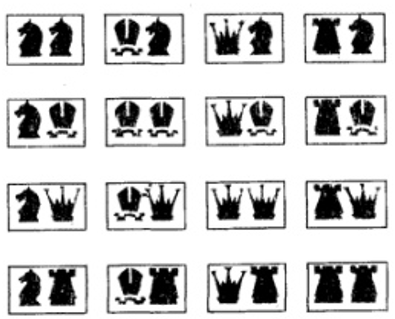
\includegraphics[width=\linewidth]{second.png}
	\footnotesize
	Рис.\,4. Существует $A^2_4 - 12$ 2-слов без повторений, составленных из элементов множеств~$N$.
\end{figure}


Поскольку первый элемент можно выбрать $n$ способами, второй тоже $n$ способами, \dots, $k$-ый тоже $n$ способами, то $k$-слово можно выбрать $n^k$ способами.

Окончательно: из $n$ элементов можно составить $n^k$ слов длины $k$.

Многие комбинаторные задачи решаются по этому правилу. Найдем, например, сколькими способами можно разделить $k$ различных предметов между $n$ людьми. Для этого расположим элементы в каком-то порядке и над каждым предметом укажем, кому он предназначается. Например, запись

\vspace{2mm}
\setlength{\extrarowheight}{3 mm}
\noindent
\begin{tabular}{|c|c|c|c|c|c|c|c|c|c|}
	\hline 1 & 1 & 3 & 2 & 2 & 1 & 2 & 3 & 3 & 1 \\ [5pt]
	\hline 1 & 2 & 3 & 4 & 5 & 6 & 7 & 8 & 9 & 10 \\ [5pt]
	\hline	
\end{tabular}
\setlength{\extrarowheight}{0 mm}

\vspace{2mm}
\noindent показывает, что первому участнику раздела достанутся 1-й, 2-й, 6-й, 10-й предметы, второму --- 4-й, 5-й, 7-й, а третьему --- 3-й, 8-й, 9-й предметы.

Мы видим, что каждый способ раздела задается $k$-словом (где $k$ - число предметов) из $n$ элементов (номеров участников раздела) Значит, число способов раздела равно $n^k$.
 % это титульный лист
\end{document}
